
%(BEGIN_QUESTION)
% Copyright 2014, Tony R. Kuphaldt, released under the Creative Commons Attribution License (v 1.0)
% This means you may do almost anything with this work of mine, so long as you give me proper credit

Suppose three different voltmeters are connected to a thermocouple, with each voltmeter having a different ambient temperature:

$$\includegraphics[width=15.5cm]{i00873x01.eps}$$

Calculate the amount of voltage registered by each of the three voltmeters, as well as answer the following questions:

\begin{itemize}
\item{} If a fourth voltmeter were connected to this same thermocouple, would it affect the readings of the other three?
\vskip 5pt
\item{} If a thermocouple transmitter were connected to this thermocouple, would it affect the readings of the voltmeters?  Would it matter whether or not this transmitter were equipped with reference junction compensation?
\end{itemize}

\underbar{file i00873}
%(END_QUESTION)





%(BEGIN_ANSWER)

Each voltmeter forms its own reference junction where the copper wires of each voltmeter connect to the chromel and alumel thermocouple wires.  Each voltmeter's reference junction produces its own voltage, opposed in polarity to the voltage of the measurement junction (at 1050 $^{o}$F).  This means we must perform a separate voltage calculation for each voltmeter based on each meter's reference junction temperature.  An equivalent schematic diagram shows how the four dissimiar metal junctions relate to one another, and to the three voltmeters:

$$\includegraphics[width=15.5cm]{i00873x02.eps}$$

The chromel and alumel wire types identify this as a {\bf type K} thermocouple, and so we may use a type K thermocouple table to look up voltages for all four junction temperatures:

\begin{itemize}
\item{} Type K at 1050 $^{o}$F = 23.439 mV
\item{} Type K at 71 $^{o}$F = 0.865 mV
\item{} Type K at 85 $^{o}$F = 1.181 mV
\item{} Type K at 60 $^{o}$F = 0.619 mV
\end{itemize}

\vskip 10pt

Since we know the measurement and reference junctions stand opposed to one another in each voltmeter loop, we may calculate each voltmeter's reading by subtracting the reference junction's voltage from the measurement junction's voltage for each voltmeter:

\vskip 10pt

\noindent
{\bf Voltage registered by the left-hand voltmeter (at 71 $^{o}$F):}

$$23.439 \hbox{ mV} - 0.865 \hbox{ mV} = 22.574 \hbox{ mV}$$

\vskip 10pt

\noindent
{\bf Voltage registered by the center voltmeter (at 85 $^{o}$F):}

$$23.439 \hbox{ mV} - 1.181 \hbox{ mV} = 22.258 \hbox{ mV}$$

\vskip 10pt

\noindent
{\bf Voltage registered by the right-hand voltmeter (at 60 $^{o}$F):}

$$23.439 \hbox{ mV} - 0.619 \hbox{ mV} = 22.820 \hbox{ mV}$$

\vskip 10pt

The voltage read by each voltmeter is a simple function of Kirchhoff's Voltage Law, with the measurement junction and the voltmeter's reference junction being the only voltage sources in the KVL loop.  Therefore, connection of a fourth voltmeter will have no effect whatsoever on the other three voltmeters.  Likewise, connection of a thermocouple transmitter to this same chromel/alumel wire pair will have no effect on the voltmeters' readings, with or without reference junction compensation.

%(END_ANSWER)





%(BEGIN_NOTES)


%INDEX% Measurement, temperature: thermocouple

%(END_NOTES)

